
\section{Απεικόνιση του ανθρώπινου σώματος}
\label{section:opengl_shading_language}

Στην εφαρμογή εκτίμησης πόζας, οι προβλέψεις του νευρωνικού δικτύου, δηλαδή το ανθρώπινο μοντέλο με την πόζα του χρήστη, πρέπει να απεικονίζονται στην οθόνη του καθρέφτη. Προς επίτευξη αυτού του σκοπού, απαιτείται μία περιγραφεί του ανθρώπινου σώματος καθώς και ενός αποδοτικού τρόπου παραγωγής των γραφικών. Έτσι, σε αυτό το κεφάλαιο θα αναλυθεί ο τρόπος χρήσης του μοντέλου \textsl{SMPL} για την μοντελοποίηση του ανθρώπινου σώματος αλλά και η χρήση της \textsl{OpenGL} για την απεικόνιση αυτού.

\subsection{SMPL: Skinned multi-person Linear Model}
\label{sec:smpl}

\begin{figure}[h]
	\centering
	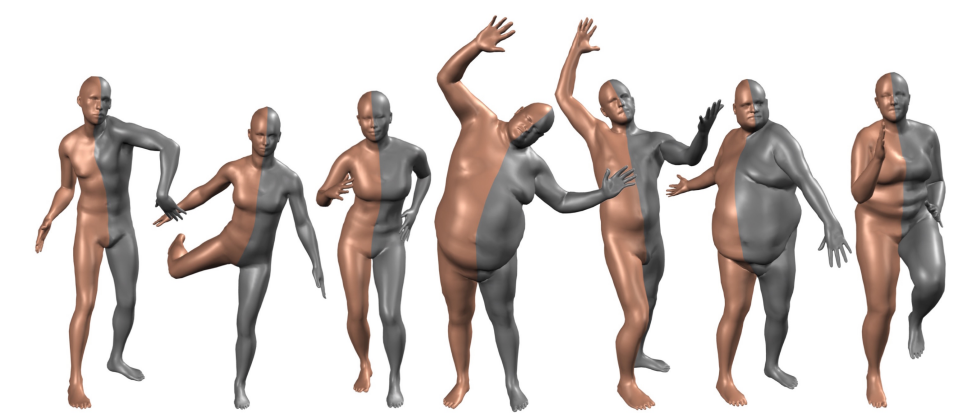
\includegraphics[scale=0.4]{images/chapter3/smpl_many_meshes.png}
	\caption{Πλέγματα ανθρώπινου σώματος με χρήση του μοντέλου SMPL}
\end{figure}

Όπως αναφέρθηκε στην ενότητα \ref{section:smpl_model}, το μοντέλο SMPL\footnote{\href{https://smpl.is.tue.mpg.de/}{https://smpl.is.tue.mpg.de/}} αποτελεί μία μοντελοποίηση του ανθρώπινου σώματος. Το ανθρώπινο σώμα θεωρείται ότι αποτελείται από την μορφή, η διαφορά των σωμάτων σε ύψος, πάχος και αναλογίες σώματος, και την πόζα, δηλαδή τον τρόπο με τον οποίο παραμορφώνεται το σώμα με την κίνηση των αρθρώσεων. Η μορφή του σώματος περιγράφεται από τις παραμέτρους $\vec{\beta} \in \mathbb{R}^{10}$. Αντίστοιχα, η πόζα περιγράφεται από τις παραμέτρους $\vec{\theta} \in \mathbb{R}^{3K}$, οι οποίες είναι οι σχετικές 3D περιστροφές των $K = 23$ αρθρώσεων σε αναπαράσταση άξονα-γωνίας. Το μοντέλο SMPL, $M(\vec{\theta},\vec{\beta}) \in \mathbb{R}^{3 \times N}$, είναι μια διαφορική συνάρτηση όπου με είσοδο τις παραμέτρους $\vec{\beta}$ και $\vec{\theta}$ παράγει ένα τριγωνικό πλέγμα του ανθρώπινου σώματος με $Ν = 6980$ κορυφές. Αυτό προκύπτει από την διαμόρφωση των κορυφών αναφοράς σύμφωνα με τις παραμέτρους $\vec{\beta}$ και $\vec{\theta}$, στην συνέχεια περιστρέφοντας τις αρθρώσεις σύμφωνα με τα $\vec{\theta}$ από την πόζα αναφοράς με χρήση του μπροστινού κινηματικού μοντέλου, και τέλος παραμορφώνοντας την επιφάνεια με γραμμική μίξη του δέρματος. Επιπλέον, το μοντέλο παράγει τα 3D σημεία κλειδιά του ανθρώπινου σκελετού (βλ. ενότητα \ref{section:skeleton_model}), $X(\vec{\theta},\vec{\beta}) \in \mathbb{R}^{3 \times P}$, υπολογίζοντας τα με γραμμική παλινδρόμηση από τις τελικές κορυφές του πλέγματος.

Στην εφαρμογή εκτίμησης πόζας, η έξοδος του βαθιού νευρωνικού δικτύου είναι το σύνολο των παραμέτρων του μοντέλου \textsl{SMPL}, $\vec{\beta}$ και $\vec{\theta}$, και εξ' ακολούθως το πλήρες ανθρώπινο πλέγμα αλλά και ο σκελετός. Με αυτό τον τρόπο, καθιστάτε δυνατή η λεπτομερής απεικόνιση του ανθρώπινου σώματος στην οθόνη παρέχοντας πολύ καλύτερη γραφική διεπαφή για τον χρήστη, τόσο για αισθητικούς όσο και για πρακτικούς λόγους, που δεν θα ήταν δυνατό να επιτευχθεί μόνο με μια μοντελοποίηση σκελετού.

Επιπλέον, το μοντέλο SMPL είναι ευέλικτο και ιδανικό για εφαρμογές όπου η απεικόνιση του σώματος είναι υψίστης σημασίας. Αναλυτικότερα, οι παράμετροι πόζας $\vec{\beta}$, όντας οι σχετικές 3D γωνίες περιστροφής των αρθρώσεων, υφίσταται εύκολη επεξεργασία για τον καθορισμό της πόζας. Ταυτόχρονα, το τελικό ανθρώπινο πλέγμα μπορεί να χρησιμοποιηθεί απευθείας για απεικόνιση στην οθόνη, με χρήση για παράδειγμα της OpenGL, μπορεί να γίνει επεξεργασία και την μορφή και την όψη του, και τελικά να ενσωματωθεί εύκολα με τα υπόλοιπα γραφικά της εφαρμογής.


\subsection{OpenGL Shading Language ES}
Όπως αναφέρθηκε παραπάνω, για την απεικόνιση του ανθρώπινου σώματος απαιτείται η απεικόνιση σύνθετων τρισδιάστατων πλεγμάτων. Τοιουτοτρόπως, για την απεικόνιση στην οθόνη χρησιμοποιούνται οι χαμηλότερου επιπέδου εντολές της OpenGL μέσω της διεπαφής προγραμματισμού που παρέχει το Kivy. Πιο συγκεκριμένα, για τον προσδιορισμό της θέσης, του χρώματος και του φωτισμού της κάθε κορυφής του πλέγματος χρησιμοποιείται η γλώσσα προγραμματισμού OpenGL Shading Language για Ενσωματώμενα Συστήματα (εν συντομία \textsl{GLSL ES})\footnote{\href{https://www.khronos.org/opengles/}{https://www.khronos.org/opengles/}}.

H \textsl{GLSL ES} είναι μία διεπαφή προγραμματισμού εφαρμογής (Application Programming Interface, εν συντομία \textsl{API}) σκίασης υψηλού επιπέδου, αποτελώντας ένα υποσύνολο της OpenGL, και παρέχει παρόμοια σύνταξη και συναρτήσεις με την γλώσσα προγραμματισμού C. To API επιτρέπει τον προγραμματισμό του καταχωρητή απόδοσης των πίξελ στην οθόνη, του \textsl{framebuffer} όπως αναλύθηκε στην ενότητα \ref{section:opengl_framebuffer}. Χαρακτηριστικό της \textsl{GLSL ES}, που την κάνει ιδανική για παραγωγή γραφικών σε ενσωματωμένα συστήματα, αποτελεί η ανεξαρτησία της από την εκάστοτε γλώσσα προγραμματισμού, η διαπλατφορμικότητα της αλλά και η απλοϊκότητα της στα στάδια παραγωγής γραφικών.

Tα επίπεδα επεξεργασίας της \textsl{GLSL ES} καθορίζονται από τους σκιαστές, οι οποίοι είναι προγράμματα που τρέχουν στην κάρτα γραφικών. Κάθε σκιαστής αντιστοιχεί σε ένα συγκεκριμένο τμήμα της διαδικασίας παραγωγής γραφικών. Επιπλέον, οι σκιαστές είναι απομονωμένοι, δηλαδή ο μόνος τρόπος επικοινωνίας μεταξύ τους είναι μέσω των εισόδων και εξόδων τους και ειδικών ομοιόμορφων μεταβλητών (uniform variables) οι οποίες είναι καθολικές και προσβάσιμες από όλους τους σκιαστές σε οποιαδήποτε φάση της διαδικασίας παραγωγής γραφικών. 

Αναλυτικότερα, στη \textsl{GLSL ES} υφίστανται δύο επίπεδα επεξεργασίας που υλοποιούνται από τον σκιαστή κορυφής (\textsl{vertex shader}) και τον σκιαστή τμήματος (\textsl{fragment shader}). 
Ο \textsl{vertex shader} δέχεται ως είσοδο μία κορυφή την φορά και τα δεδομένα σχετικά με αυτή, όπως τη θέση της στον τρισδιάστατο χώρο και το κανονικό της διάνυσμα (\textsl{vertex normal} βλ. παράρτημα \ref{definition:vertex_normal}). Η έξοδος του \textsl{vertex shader} είναι η θέση της εκάστοτε κορυφής στις συντεταγμένες της οθόνης. Από την άλλη μεριά, ο \textsl{fragment shader} δέχεται ως είσοδο τα πίξελ της οθόνης που αντιστοιχούν σε ένα πρωτόγονο σχήμα, όπως υπολογίστηκαν από τον \textsl{vertex shader}, και καθορίζει το χρώμα, το βάθος και ενδεχομένως το στένσιλ για αυτό το τμήμα.